\FloatBarrier
\subsubsection{Mediciones de ganancia y frecuencia}

La ilustración \ref{ilus:entrada-salida-inversor} muestra las mediciones de voltaje de entrada y salida del amplificador inversor.

\begin{ilustracion}[hb]
    \centering
    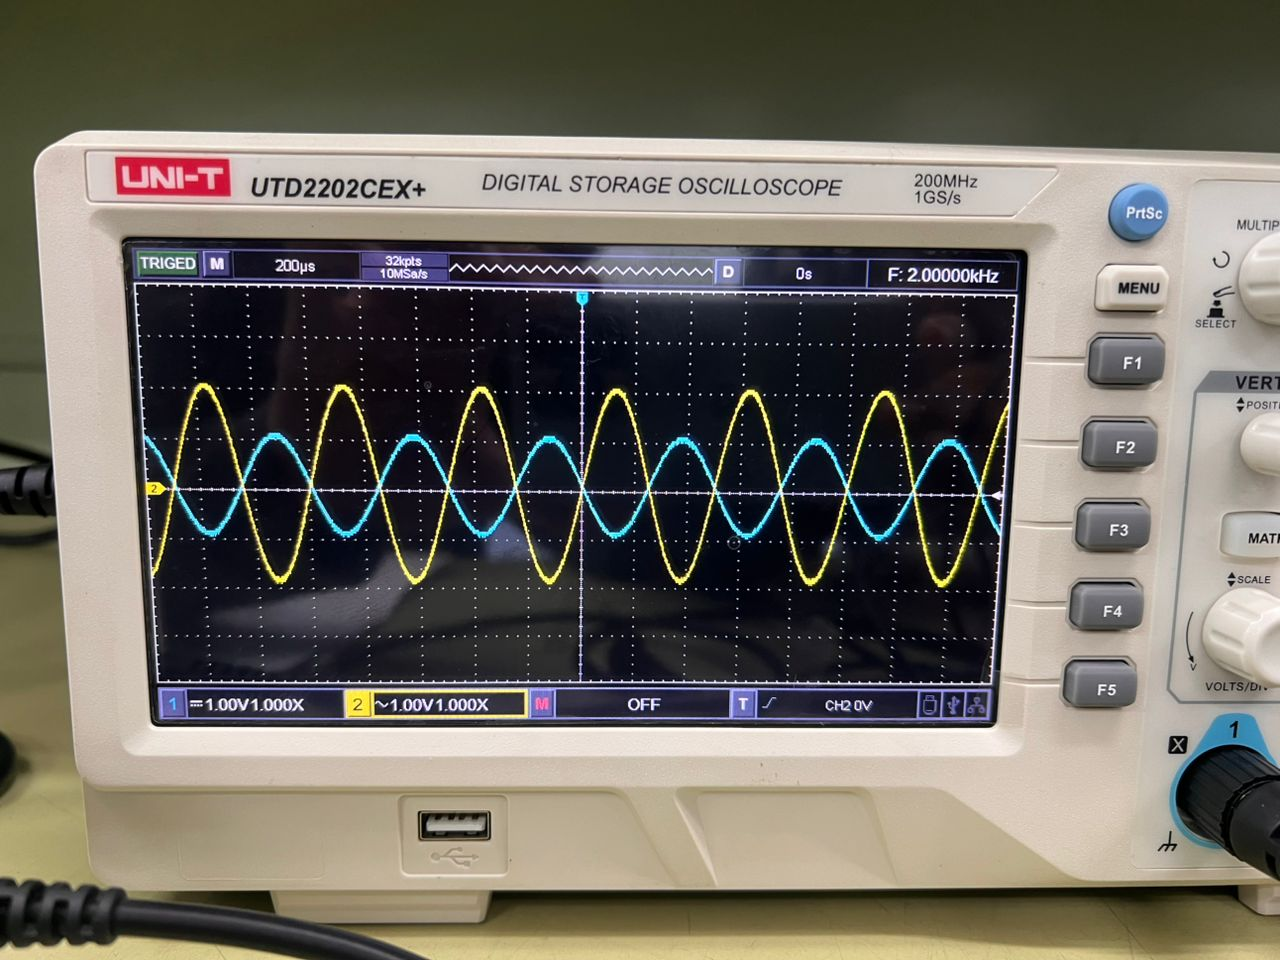
\includegraphics[width=0.8\textwidth]{resultados/inversor.jpg}
    \caption{Entrada y salida amplificador inversor.}
    \label{ilus:entrada-salida-inversor}
\end{ilustracion}

La ilustración \ref{ilus:entrada-salida-no-inversor} muestra las mediciones de voltaje de entrada y salida del amplificador no inversor.

\begin{ilustracion}[ht]
    \centering
    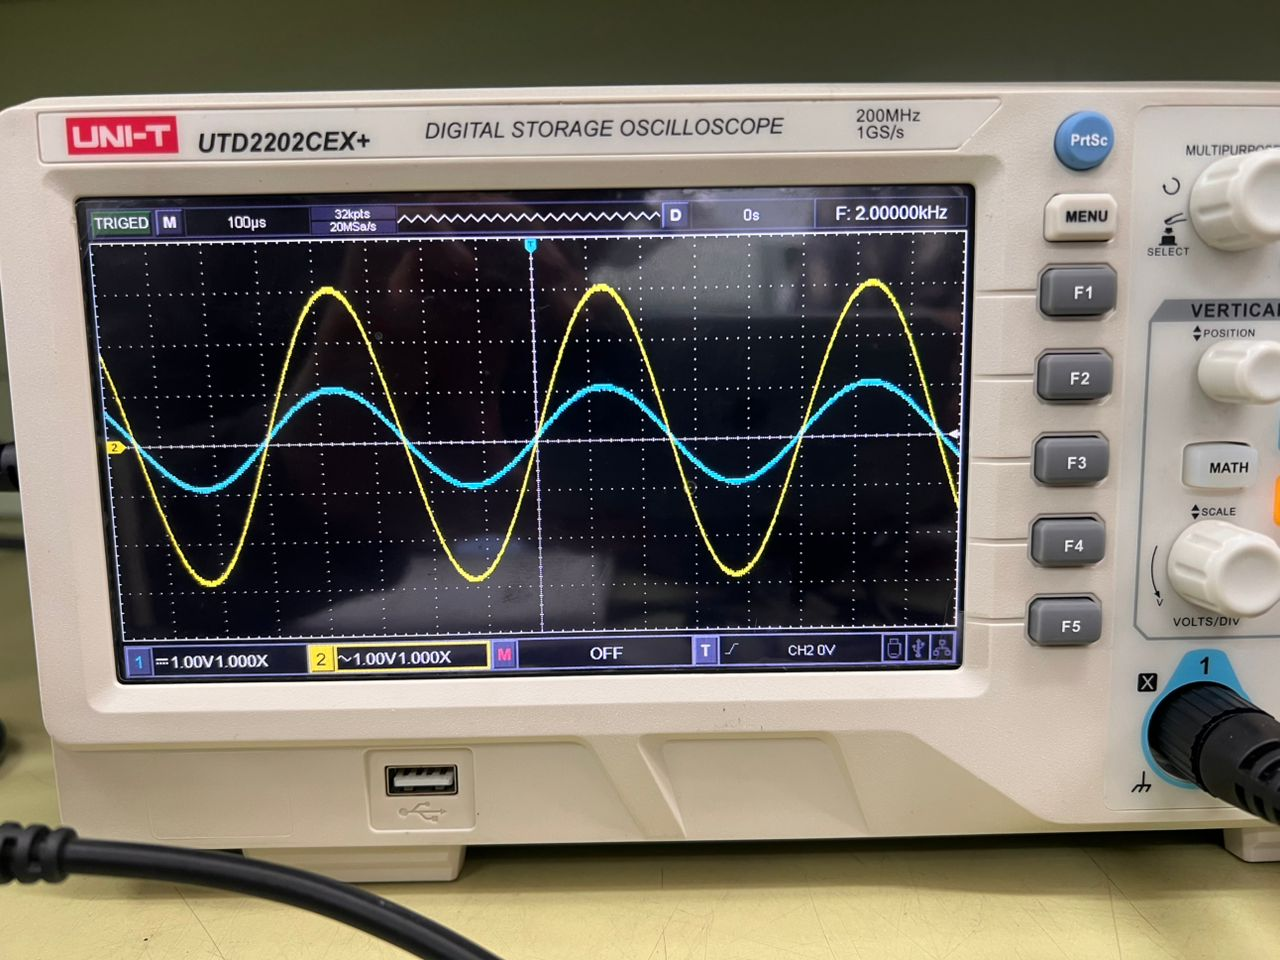
\includegraphics[width=0.8\textwidth]{resultados/no-inversor.jpg}
    \caption{Entrada y salida amplificador no inversor.}
    \label{ilus:entrada-salida-no-inversor}
\end{ilustracion}

La ilustración \ref{ilus:entrada-salida-restador} muestra las mediciones de voltaje de entrada y salida del amplificador restador.

\begin{ilustracion}[ht]
    \centering
    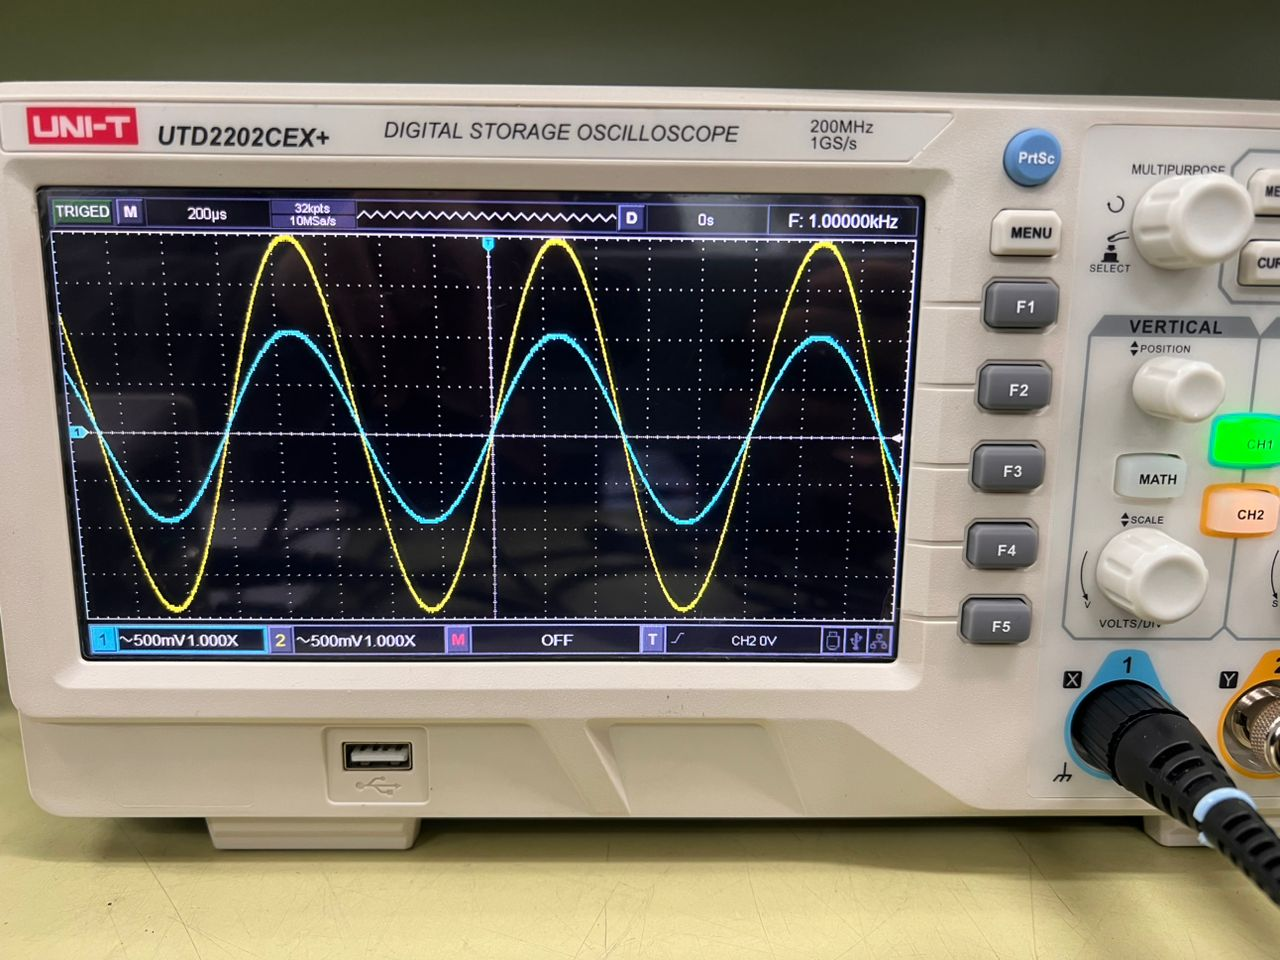
\includegraphics[width=0.8\textwidth]{resultados/restador.jpg}
    \caption{Entrada y salida amplificador restador.}
    \label{ilus:entrada-salida-restador}
\end{ilustracion}



\begin{table}[ht]
\centering
\begin{tabular}{|c|c|c|c|c|c|c|c|c|}
\hline
Topología & \(V_i(i)\) & \(\Delta V_i(i)\) & \(V_o(i)\) & \(\Delta V_o(i)\) & \(T\) (ms) & \(\Delta T\) (ms) & Ganancia & \(\Delta \text{Ganancia}\) \\ \hline
Inversor & 1         & 0.2               & -2         & 0.2               & 1.0        & 0.02              & -2.00             & 0.447 \\ \hline
No inversor & 1         & 0.2               & 3          & 0.2               & 1.0        & 0.02              & 3.00              & 0.632 \\ \hline
Restador & 0.5       & 0.22              & 2          & 0.1               & 1.0        & 0.02              & 4.00              & 1.77 \\ \hline
\end{tabular}
\caption{Ganancia topologías clásicas.}
\label{tab:resultados-ganancia-frecuencia-topologias-basicas}
\end{table}

\subsubsection{Efecto del integrador no inversor}

La ilustración \ref{ilus:entrada-salida-integrador-no-inversor} muestra las mediciones de voltaje de entrada y salida del amplificador integrador no inversor.
\begin{ilustracion}[ht]
    \centering
    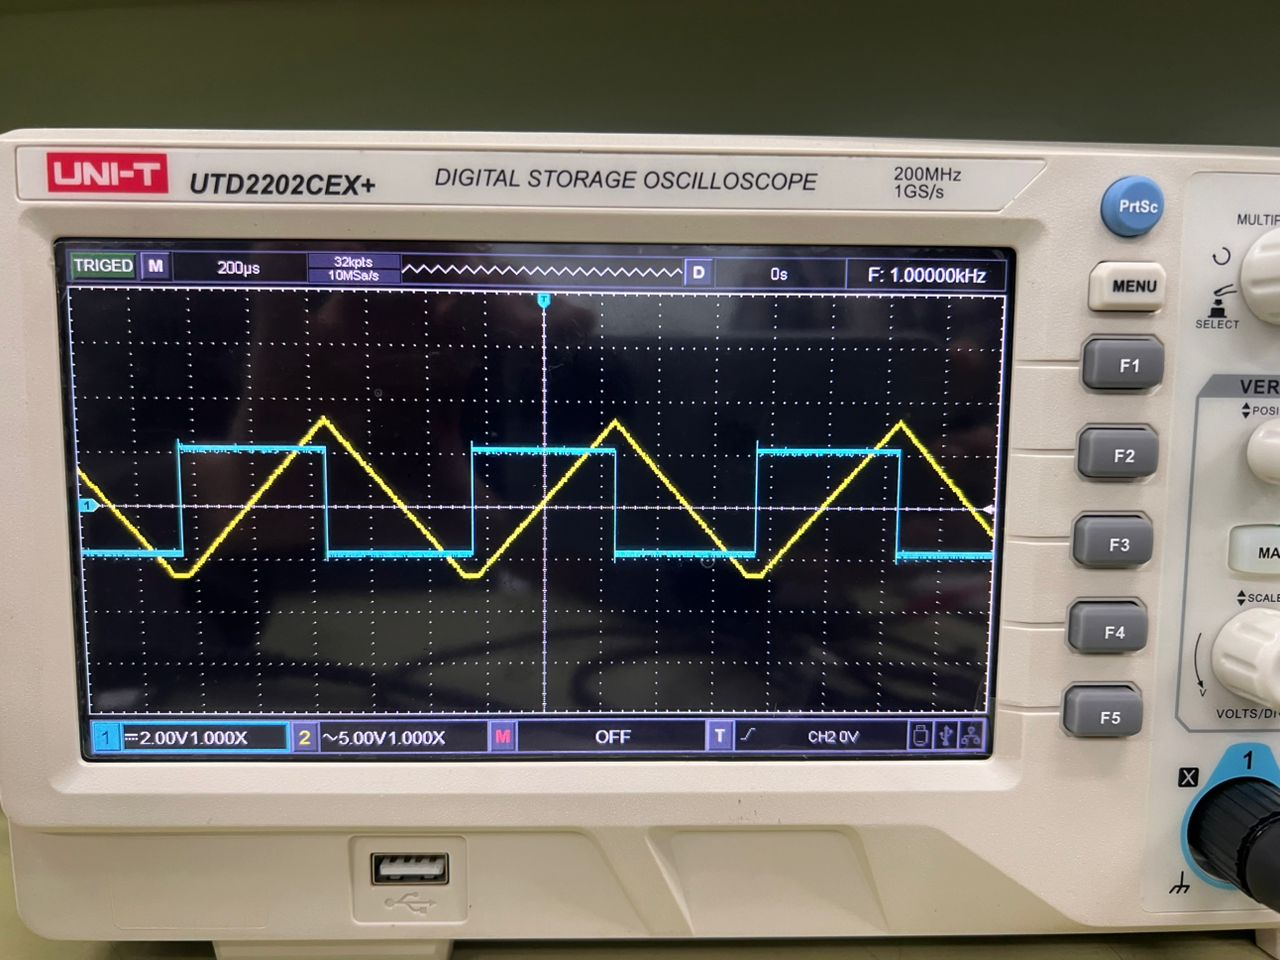
\includegraphics[width=0.8\textwidth]{resultados/integrador-no-inversor.jpg}
    \caption{Entrada vs salida amplificador integrador no inversor.}
    \label{ilus:entrada-salida-integrador-no-inversor}
\end{ilustracion}

\subsubsection{Convertidor de tensión a corriente}

El cuadro \ref{tab:medicion-voltaje-entrada-convertidor-tension-corriente} muestra la medición de voltaje de entrada del convertidor tensión-corriente.

\begin{table}[ht]
    \centering
    \begin{tabular}{|c|c|}
        \hline
        \(V_i\) & \(\Delta V_i\) \\ \hline
        5.2 & 0.4 \\ \hline
    \end{tabular}
    \caption{Medición de voltaje de entrada del convertidor tensión-corriente.}
    \label{tab:medicion-voltaje-entrada-convertidor-tension-corriente}
\end{table}

El cuadro \ref{tab:resultados-convertidor-tension-corriente} muestra las mediciones del convertidor tensión-corriente.

\begin{table}[h!]
\centering
\begin{tabular}{|c|c|c|c|c|c|}
\hline
\(V_o\) & \(\Delta V_o\) & \(R\) [$k\Omega$] & \(\Delta R\) [$k\Omega$] & I (mA) & \(\Delta I\) (mA) \\ \hline
0.05 & 0.01 & 1.000 & 0.050 & 50.00 & 10.30 \\ \hline
0.5 & 0.1 & 11.000 & 0.550 & 45.50 & 9.370 \\ \hline
1.0 & 0.1 & 22.000 & 1.100 & 45.50 & 5.080 \\ \hline
2.0 & 0.2 & 39.000 & 1.950 & 51.30 & 5.730 \\ \hline
1.3 & 0.1 & 27.000 & 1.350 & 48.10 & 4.420 \\ \hline
\end{tabular}
\caption{Mediciones del convertidor tensión-corriente.}
\label{tab:resultados-convertidor-tension-corriente}
\end{table}

